\chapter{无损编码}
\label{chap:lossless-coding}

一台设备只发出四种符号$a,b,c,d$，出现的概率分别是$0.4,0.3,0.2,0.1$。要把一长串这样的符号存成0和1，最直接的办法是每个符号用两位：$a=00$，$b=01$，$c=10$，$d=11$。可是$a$出现得最多，$d$出现得最少，让$a$用一位、让$d$用三位，平均下来能不能少于两位？能少多少？少到什么程度就不可能再少？

第一个困难是还原。码字长短不一以后，接收方看到的是一串没有分隔符的0和1，要自己找出每个码字从哪里开始、到哪里结束。有的码表单看每个码字都互不相同，拼起来却会产生歧义。第二个困难是衡量。省下来的长度是按概率加权的平均，单条消息可能变长；而且平均能省多少，要与源分布的熵比较，熵的定义来自第~\ref{chap:information-measures}章。

本章先写清编码模型和评价量，再研究码表需要满足什么条件才能被唯一地拆开，由此得到码长必须满足的Kraft–McMillan不等式。有了这个约束，平均码长的下界就是熵，按自信息取整的码长又能使平均码长小于熵加一。

随后构造两种具体编码：Huffman编码对给定的符号表求出平均码长最短的前缀码，算术编码把整条消息对应到一个小区间。最后把符号组成长块：要求零错误时，变长块编码使每符号的冗余按块长的倒数减小；允许小概率出错时，只给高概率的块编号就能以接近熵的定长码率传输。两种方式共享熵这个极限，但付出的资源与承担的风险不同，第~\ref{sec:lossless-finite-resources}节在有限块长和模型失配下比较它们。

全章用到第~\ref{chap:information-measures}章的熵与自信息、第~\ref{chap:distribution-comparison}章的KL散度及其非负性，以及第~\ref{chap:laws-of-large-numbers}章的弱大数律。本部分的对数都以$2$为底，信息量的单位是bit。

\section{编码模型}
\label{sec:lossless-model}

“用较少的0和1记录消息”要变成数学问题，得先说清四件事：消息从哪里来，编码把什么映射成什么，解码要恢复什么，以及“较少”按什么标准计算。本节依次固定这些约定，并引入贯穿全章的四符号例子。

\paragraph{信源与消息}
设$\mathcal{X}$是有限集合，称为\term{字母表}（alphabet）。\term{信源}（source）是取值于$\mathcal{X}$的随机变量$X$，其概率质量函数记作
\[
 p(x)=\mathbb{P}(X=x),\qquad x\in\mathcal{X}.
\]
信源连续发出$n$个符号时，得到长度为$n$的消息$X_{1:n}=(X_1,\dots,X_n)$，它的取值记作$x_{1:n}$。本章除非特别说明，都假设$X_1,X_2,\dots$独立同分布，每个都服从$p$，于是
\begin{equation}
 \mathbb{P}(X_{1:n}=x_{1:n})=p(x_{1:n})=\prod_{i=1}^{n}p(x_i).
 \label{eq:lossless-product}
\end{equation}
这里$p(x_{1:n})$是长度为$n$的消息的概率，用同一个字母$p$记，参数的形状说明它指哪一个。

概率为零的符号永远不会出现，对平均量也没有贡献。本章约定把它们从字母表中去掉，即$p(x)>0$对每个$x\in\mathcal{X}$成立；需要讨论“设计时以为某个符号不会出现”的情形时（第~\ref{sec:lossless-arithmetic}小节和第~\ref{sec:lossless-finite-resources}节），再单独说明。

\paragraph{码字与编码}
记$\{0,1\}^{*}$为所有有限长二进制串的集合，其中包括长度为零的空串。二进制串$s$的长度记作$\lvert s\rvert$。一个\term{二进制码}（binary code）是映射
\[
 c:\mathcal{X}\to\{0,1\}^{*},
\]
$c(x)$称为符号$x$的\term{码字}（codeword），$\ell(x)=\lvert c(x)\rvert$称为它的码长。逐符号编码一条消息时，把各符号的码字依次拼接起来，
\begin{equation}
 c(x_{1:n})=c(x_1)c(x_2)\cdots c(x_n),
 \label{eq:lossless-extension}
\end{equation}
这个映射称为\term{码的扩展}（extension of a code）。\term{编码器}（encoder）执行这一映射，\term{解码器}（decoder）从收到的二进制串恢复消息。

\paragraph{贯穿全章的例子}
取$\mathcal{X}=\{a,b,c,d\}$，概率表为
\[
 p(a)=0.4,\quad p(b)=0.3,\quad p(c)=0.2,\quad p(d)=0.1 .
\]
码表取$a\mapsto0$、$b\mapsto10$、$c\mapsto110$、$d\mapsto111$。消息$abac$编码成
\[
 c(abac)=0\;10\;0\;110=0100110,
\]
共$7$位，比每符号两位的定长码少$1$位。解码器从左往右读：读到$0$就是$a$；读到$10$就是$b$；再读到$0$是$a$；最后$110$是$c$。图~\ref{fig:lossless-coding-model}画出这一过程。为什么这张码表能这样一步步读出来，是第~\ref{sec:lossless-decodability}节的问题。

\begin{BookInlineFigure}
 \centering
 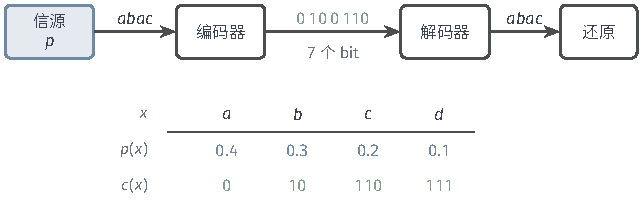
\includegraphics[width=108mm]{figures/07-probability/05-source-coding/tikz/lossless-coding-model/figure.pdf}
 \caption{无损编码的模型。信源（蓝框）按概率表$p$发出消息$abac$，编码器按下方码表把每个符号换成码字并依次拼接（绿色），得到$7$位二进制串；解码器从二进制串精确恢复出同一条消息。}
 \label{fig:lossless-coding-model}
\end{BookInlineFigure}

\paragraph{逐符号与整块，变长与定长}
上面的码表一次处理一个符号，称为逐符号编码。也可以先把$n$个符号组成一块，把整块$x_{1:n}$看成字母表$\mathcal{X}^n$中的一个“大符号”，直接给它分配码字，这就是\term{块编码}（block coding）。整块编码时，被编码的字母表从$\lvert\mathcal{X}\rvert$个元素变成$\lvert\mathcal{X}\rvert^n$个元素，码表的规模随之增长。

码字长度也有两种安排。所有码字等长的称为\term{定长码}（fixed-length code），例如每符号两位的码，或者给每个长度为$n$的块分配同样多位的码；码字长度可以不同的称为\term{变长码}（variable-length code）。定长码不需要寻找码字边界，按固定位数切开即可；变长码要靠码表本身的结构来确定边界。

\paragraph{解码恢复什么}
无损编码要求精确还原，但“还原什么”需要约定。逐符号编码时，解码器要从拼接串$c(x_{1:n})$恢复整条符号序列$x_{1:n}$，而不仅是某一个符号。整块编码时，解码器恢复的是块$x_{1:n}$本身。另一个必须事先约定的是消息长度：解码器是否事先知道$n$，还是要从二进制串本身判断消息在哪里结束。这两种约定的差别在第~\ref{sec:lossless-average-length}节处理确定源时、在第~\ref{sec:lossless-arithmetic}小节处理算术编码的终止时都会出现。

\paragraph{三个评价量}
衡量一个编码方案时，本章分别使用三个量。第一个是按信源概率加权的\term{平均码长}（expected code length），
\begin{equation}
 L(c)=\mathbb{E}[\ell(X)]=\sum_{x\in\mathcal{X}}p(x)\ell(x),
 \label{eq:lossless-average-length}
\end{equation}
它回答长期平均每个符号用多少位：由第~\ref{chap:laws-of-large-numbers}章的大数律，独立编码$n$个符号的总位数除以$n$趋于$L(c)$。第二个是最坏码长$\max_{x}\ell(x)$，它决定缓冲区要准备多大、单条消息最多会多长。第三个是还原错误概率，即解码结果与原消息不同的概率。

三个量回答不同的问题。例中变长码的平均码长是
\[
 L(c)=0.4\times1+0.3\times2+0.2\times3+0.1\times3=1.9 ,
\]
比定长码的$2$少；但最坏码长是$3$，比定长码的$2$多。消息$ddd$用变长码要$9$位，用定长码只要$6$位。所以变长码的“节省”只是平均意义上的，第~\ref{sec:lossless-decodability}节至第~\ref{sec:lossless-methods}节都要求错误概率为零、以平均码长为主要指标，第~\ref{sec:lossless-block-limits}节再允许错误概率为正但趋于零，换取定长的码字。


\section{可解码约束}
\label{sec:lossless-decodability}

码字各不相同，是不是就够了？看下面这张码表：
\[
 a\mapsto0,\qquad b\mapsto010,\qquad c\mapsto01,\qquad d\mapsto10 .
\]
四个码字互不相同，单独收到任何一个码字都能认出是哪个符号。可是收到拼接串$010$时，它既可以是$b$，也可以是$ca$（$01$接$0$），还可以是$ad$（$0$接$10$）。图~\ref{fig:lossless-ambiguous-parse}画出这三种切法。接收方没有分隔符，无法判断发送的是哪一条消息。

\begin{BookInlineFigure}
 \centering
 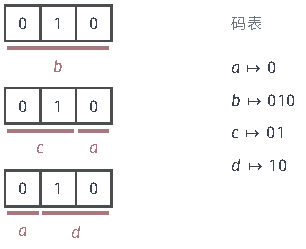
\includegraphics[width=52mm]{figures/07-probability/05-source-coding/tikz/lossless-ambiguous-parse/figure.pdf}
 \caption{码字互不相同、拼接后却有歧义的码。右侧为码表；同一个收到的串$010$（方框）有三种切分方式，红色横线下方是每段对应的符号，分别解读为$b$、$ca$和$ad$。}
 \label{fig:lossless-ambiguous-parse}
\end{BookInlineFigure}

所以要区分两层要求。码$c$称为\term{非奇异码}（nonsingular code），如果不同符号的码字不同，即$c$作为$\mathcal{X}\to\{0,1\}^{*}$的映射是单射。真正需要的是更强的一层：

\begin{definition}[唯一可译码]
\label{def:lossless-uniquely-decodable}
若码$c$的扩展~\eqref{eq:lossless-extension}在所有有限长符号序列上是单射，即对任意$m,n\geq1$与$x_{1:m}\in\mathcal{X}^m$、$y_{1:n}\in\mathcal{X}^n$，
\begin{equation}
 c(x_1)\cdots c(x_m)=c(y_1)\cdots c(y_n)\ \Longrightarrow\ m=n,\ x_{1:m}=y_{1:n},
 \label{eq:lossless-ud}
\end{equation}
则称$c$为\term{唯一可译码}（uniquely decodable code）。
\end{definition}

条件里$m$与$n$可以不同，这是为了把“同一个串能否被切成不同个数的码字”也排除掉。上面的例子中$010$一次切成一个码字、一次切成两个码字，所以那张码表非奇异却不唯一可译。唯一可译码中不能有空码字：若$c(x)$是空串，则$c(x)$与$c(xx)$相同，违反式~\eqref{eq:lossless-ud}。

唯一可译性只说“原则上能切开”，没说怎样切、要往后看多远。下面先看一类可以边读边切的码，再研究所有唯一可译码对码长的共同限制。

\subsection{前缀码}
\label{sec:lossless-prefix-codes}

开头例子的歧义来自一个码字是另一个码字的开头：$0$是$01$和$010$的开头，$01$又是$010$的开头。读到$0$时，解码器不知道这个码字是否已经结束。如果禁止这种情况，读到一个完整码字时就能立刻断开。

\begin{definition}[前缀码]
\label{def:lossless-prefix-code}
若串$s$可写成$s=ut$，则称$u$是$s$的前缀。若码$c$中没有一个码字是另一个码字的前缀，则称$c$为\term{前缀码}（prefix code），也称即时码。
\end{definition}

\paragraph{码树}
二进制串可以画在一棵二叉树上：从根出发，读到$0$走左支，读到$1$走右支，每个串对应一个结点，串长就是结点的深度。码字是树上的一些结点，从根到这些结点的路径合在一起称为\term{码树}（code tree）。“$u$是$s$的前缀”就是“结点$u$在根到结点$s$的路径上”。因此前缀码的码字恰好都是码树的叶结点：没有一个码字结点在另一个码字结点的下方。

图~\ref{fig:lossless-prefix-tree}(a)是贯穿例的码$0,10,110,111$。四个码字都是叶结点，所以它是前缀码。图中(b)是另一张码表$0,01,011,111$，码长同样是$1,2,3,3$，但$a$的码字$0$位于$b$的码字$01$上方，$01$又位于$011$上方，所以它不是前缀码。

\begin{BookInlineFigure}
 \centering
 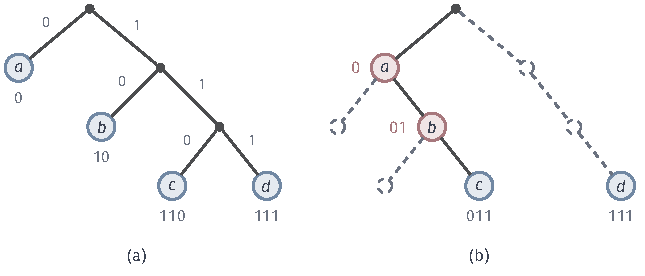
\includegraphics[width=110mm]{figures/07-probability/05-source-coding/tikz/lossless-prefix-tree/figure.pdf}
 \caption{码字作为二叉树的结点，左支读$0$、右支读$1$，结点下方或左侧是它的码字。(a)前缀码$0,10,110,111$，四个码字（蓝圈）都是叶结点。(b)码$0,01,011,111$，码长相同，但$a,b$的码字（红圈）位于其他码字的路径上；虚线和虚圈是路径经过的、不对应码字的结点。}
 \label{fig:lossless-prefix-tree}
\end{BookInlineFigure}

\paragraph{即时解码}
前缀码的解码过程是在码树上行走：从根出发，按收到的位逐步向下，到达叶结点就输出对应符号，然后回到根继续。到达叶结点时，这个码字一定已经结束，因为叶结点下面没有别的码字；而在到达叶结点之前，当前读到的串不是任何码字，也不可能提前断开。

用图~\ref{fig:lossless-prefix-tree}(a)解码$0100110$：读$0$到达叶$a$，输出$a$；读$1,0$到达叶$b$，输出$b$；读$0$输出$a$；读$1,1,0$到达叶$c$，输出$c$。每次输出都在读完该码字最后一位的那一刻完成，不需要看后面的位，这就是“即时”一词的含义。

\begin{theorem}[前缀码唯一可译]
\label{thm:lossless-prefix-ud}
前缀码是唯一可译码。
\end{theorem}

\begin{proof}
设$c(x_1)\cdots c(x_m)=c(y_1)\cdots c(y_n)$，记这个共同的串为$s$。$c(x_1)$与$c(y_1)$都是$s$的前缀，所以较短的一个是较长的一个的前缀。前缀码中这只能在两者相同时发生，于是$c(x_1)=c(y_1)$。前缀码中码字互不相同，所以$x_1=y_1$。

从$s$的两边去掉这个共同的码字，剩下的串仍满足同样的等式，对剩余部分重复上面的论证。每一步去掉同一个码字，直到某一边先用完。若$m<n$，左边用完时剩下的串是空串，右边却还有非空码字$c(y_{m+1})\cdots c(y_n)$；前缀码不含空码字，这不可能，因为空串是任何码字的前缀。所以$m=n$，且各位置的符号都相同。
\end{proof}

\paragraph{唯一可译但不是前缀码}
反过来不成立。图~\ref{fig:lossless-prefix-tree}(b)的码$a\mapsto0$、$b\mapsto01$、$c\mapsto011$、$d\mapsto111$不是前缀码，却是唯一可译码。把每个码字倒过来读，得到$0,10,110,111$，这正是(a)中的前缀码。收到整串后从右向左读，就是在倒序码的码树上即时解码，所以拼接串只有一种切法。

这张码的代价是解码延迟。设收到的串以$0$开头、后面跟着一串$1$。若串在$0111$处结束，它是$ad$；若是$01111$，它是$bd$；若是$011111$，它是$cd$；若是$0111111$，又回到$a$后接两个$d$。第一个码字是$0$、$01$还是$011$，取决于后面$1$的个数除以$3$的余数，解码器必须等这一串$1$全部结束才能确定第一个符号。前缀码没有这种等待，所以实际中几乎总用前缀码；下一小节说明，从码长的角度看，用前缀码也没有任何损失。

\subsection{Kraft–McMillan不等式}
\label{sec:lossless-kraft}

码长越短越好，但不能任意短：$\mathcal{X}$有四个符号，就不可能都用长度$1$的码字，因为长度为$1$的二进制串只有两个。一般地，码长受什么限制？下面先就前缀码回答，再把结论推广到全部唯一可译码。

\paragraph{码字占用的区间}
把码字$s=s_1s_2\cdots s_\ell$看成二进制小数$0.s_1s_2\cdots s_\ell$，它对应$[0,1)$中的区间
\[
 I(s)=\bigl[\,0.s_1\cdots s_\ell,\ 0.s_1\cdots s_\ell+2^{-\ell}\bigr),
\]
即所有以$s$开头的无限二进制展开所组成的数。区间的长度是$2^{-\ell}$：码字越短，占用的区间越长。在码树上，$I(s)$就是结点$s$下面整棵子树的“影子”。

两个码字$u,s$中若$u$是$s$的前缀，则$I(s)\subset I(u)$；若彼此都不是对方的前缀，则两者在某一位上第一次出现不同，一个在那一位取$0$、另一个取$1$，于是$I(u)$与$I(s)$不相交。所以前缀码的码字对应$[0,1)$中两两不交的区间。图~\ref{fig:lossless-kraft-intervals}第一行是贯穿例的码，四个区间恰好铺满$[0,1)$。

\begin{theorem}[Kraft不等式]
\label{thm:lossless-kraft}
设$\mathcal{X}=\{x_1,\dots,x_m\}$，正整数$\ell_1,\dots,\ell_m$。存在码长为$\ell_1,\dots,\ell_m$的二进制前缀码，当且仅当
\begin{equation}
 \sum_{i=1}^{m}2^{-\ell_i}\leq1 .
 \label{eq:lossless-kraft}
\end{equation}
\end{theorem}

\begin{proof}
必要性。前缀码的码字对应$[0,1)$中两两不交的区间，它们的长度之和不超过$[0,1)$的长度$1$，这就是式~\eqref{eq:lossless-kraft}。

充分性。把码长重新编号使$\ell_1\leq\ell_2\leq\cdots\leq\ell_m$，并令
\[
 F_1=0,\qquad F_i=\sum_{j<i}2^{-\ell_j}\quad(i=2,\dots,m).
\]
由式~\eqref{eq:lossless-kraft}，$F_i<1$。每个$2^{-\ell_j}$（$j<i$）都是$2^{-\ell_i}$的整数倍，所以$F_i$也是$2^{-\ell_i}$的整数倍，它的二进制展开在第$\ell_i$位之后全是$0$。取第$i$个码字为$F_i$二进制展开的前$\ell_i$位，于是
\[
 I(c(x_i))=\bigl[F_i,\,F_i+2^{-\ell_i}\bigr)=\bigl[F_i,\,F_{i+1}\bigr) ,
\]
这里$F_{m+1}=\sum_j2^{-\ell_j}\leq1$。这些区间首尾相接、两两不交。若某个码字$u$是另一个码字$s$的前缀，则$I(s)\subset I(u)$，与不交矛盾。所以得到的码是前缀码。
\end{proof}

充分性的证明给出了构造方法：码长从短到长排好，依次在$[0,1)$中从左往右截取长$2^{-\ell_i}$的区间。图~\ref{fig:lossless-kraft-intervals}第二行把这个方法用于码长$2,2,3,4$。依次得到
\[
 F_1=0,\quad F_2=\tfrac14,\quad F_3=\tfrac12,\quad F_4=\tfrac58 ,
\]
码字为$00,01,100,1010$。四个区间只占了$[0,1)$的$11/16$，剩下的$[11/16,1)$没有用上：这组码长满足Kraft不等式但不取等号，说明还有缩短码字的余地，例如把$1010$缩短为$101$仍是前缀码。

\begin{BookInlineFigure}
 \centering
 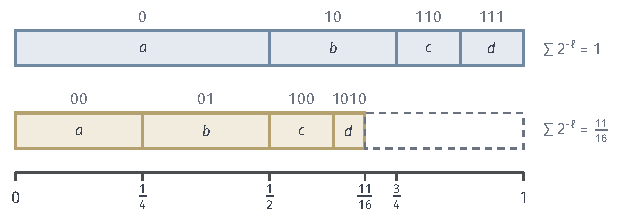
\includegraphics[width=106mm]{figures/07-probability/05-source-coding/tikz/lossless-kraft-intervals/figure.pdf}
 \caption{码字作为$[0,1)$中的二进区间，长度为$\ell$的码字占用长$2^{-\ell}$的区间，区间上方是码字。第一行（蓝）为码$0,10,110,111$，区间铺满$[0,1)$，Kraft和等于$1$。第二行（黄）为码长$2,2,3,4$按充分性证明构造的码$00,01,100,1010$，区间占去$11/16$，虚线框为未用的部分。}
 \label{fig:lossless-kraft-intervals}
\end{BookInlineFigure}

\paragraph{推广到唯一可译码}
唯一可译码的码字可以互为前缀，区间就可能嵌套，上面的必要性证明不再适用。可是码长仍然受同样的限制。McMillan的证明换了一个角度：不看单个码字，而是看把$k$个码字拼起来以后能得到多少种不同的串。

\begin{theorem}[McMillan不等式]
\label{thm:lossless-mcmillan}
任何二进制唯一可译码的码长都满足式~\eqref{eq:lossless-kraft}。
\end{theorem}

\begin{proof}
记$K=\sum_{x\in\mathcal{X}}2^{-\ell(x)}$，$\ell_{\max}=\max_x\ell(x)$。唯一可译码没有空码字，所以每个$\ell(x)\geq1$。固定正整数$k$，把$K$的$k$次方展开：
\[
 K^k=\sum_{x_1\in\mathcal{X}}\cdots\sum_{x_k\in\mathcal{X}}2^{-(\ell(x_1)+\cdots+\ell(x_k))}.
\]
求和的每一项对应一条长度为$k$的符号序列$x_{1:k}$，指数中的和正是它的码串$c(x_{1:k})$的长度。按码串长度$s$分组，记$N_s$为码串长度恰为$s$的序列个数，则
\[
 K^k=\sum_{s=k}^{k\ell_{\max}}N_s\,2^{-s}.
\]
唯一可译性说明不同的序列$x_{1:k}$给出不同的码串，而长度为$s$的二进制串只有$2^s$个，所以$N_s\leq2^s$。代入上式，每一项不超过$1$，项数为$k\ell_{\max}-k+1$，于是
\begin{equation}
 K^k\leq k(\ell_{\max}-1)+1 .
 \label{eq:lossless-mcmillan-count}
\end{equation}
若$K>1$，左边随$k$指数增长，右边只线性增长，$k$足够大时不等式必然被破坏。所以$K\leq1$。
\end{proof}

这个证明的直观是计数。若$K>1$，长序列的数目会比可用的二进制串增长得更快，迟早有两条序列不得不共用同一个码串。图~\ref{fig:lossless-mcmillan-growth}用码长$1,1,2$作例子，此时$K=1.25$。式~\eqref{eq:lossless-mcmillan-count}的右边为$k+1$，从$k=12$起$1.25^{k}$超过它。具体地，$1.25^{12}\approx14.55>13$：长度为$12$的符号序列给出的码串数目，已经超出了相应长度的二进制串所能容纳的数目，这三个码长不可能属于任何唯一可译码。

\begin{BookInlineFigure}
 \centering
 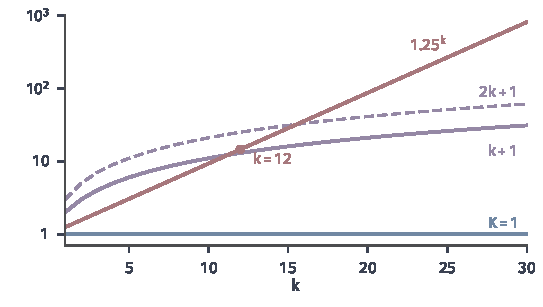
\includegraphics[width=92mm]{figures/07-probability/05-source-coding/matplotlib/lossless-mcmillan-growth/figure.pdf}
 \caption{McMillan计数论证，纵轴为对数坐标。红线为码长$1,1,2$的$K^k=1.25^k$，紫色实线为$\ell_{\max}=2$时的上界$k+1$，二者在红点$k=12$处交叉；紫色虚线为$\ell_{\max}=3$时的上界$2k+1$。蓝线为满足等号的码长$1,2,3,3$，$K^k=1$始终在上界之下。}
 \label{fig:lossless-mcmillan-growth}
\end{BookInlineFigure}

定理~\ref{thm:lossless-kraft}与定理~\ref{thm:lossless-mcmillan}合起来称为\term{Kraft–McMillan不等式}（Kraft–McMillan inequality）：任何唯一可译码的码长满足式~\eqref{eq:lossless-kraft}，而满足式~\eqref{eq:lossless-kraft}的码长都能由前缀码实现。因此，凡是只依赖码长的指标，例如平均码长，在唯一可译码中能达到的值，用前缀码都能达到。前面那张倒序的唯一可译码$0,01,011,111$没有带来任何码长上的好处，只多了解码延迟。

\paragraph{充分性说的是码长}
定理~\ref{thm:lossless-kraft}的充分性只保证“存在”一个具有这些码长的前缀码，并不说任何一种具有这些码长的码字分配都可以唯一解码。码长$1,2,2$满足
\[
 2^{-1}+2^{-2}+2^{-2}=1 ,
\]
按构造得到前缀码$0,10,11$。若随手把码字取成$0,00,11$，码长相同，但$00$既可以是第二个符号，也可以是第一个符号出现两次，不唯一可译。码长合格之后，码字仍要按证明中的方法（或其他保证前缀性的方法）来分配。


\section{平均码长}
\label{sec:lossless-average-length}

Kraft–McMillan不等式说明码长不能都很短：给一个符号分配短码字，就占去了$[0,1)$中一段长区间，留给其他符号的空间随之变小。现在把信源的概率加进来，问：在唯一可译的要求下，平均码长$L(c)$最小能到多少？

\paragraph{熵与自信息}
回答要用到第~\ref{chap:information-measures}章的两个量，这里按本部分的约定以$2$为底重新写出。符号$x$的自信息是$-\log_2p(x)$，单位为bit；信源的熵是自信息的平均，
\begin{equation}
 H(X)=-\sum_{x\in\mathcal{X}}p(x)\log_2p(x).
 \label{eq:lossless-entropy}
\end{equation}
第~\ref{chap:information-measures}章以自然对数计量，单位为nat；以nat计的熵除以$\ln2$，就得到这里以bit计的值。熵是“平均要问几个是非题才能确定结果”：若$p$是均匀分布，$\lvert\mathcal{X}\rvert=2^k$，则恰好需要$k$个是非题，此时$H(X)=k$。

贯穿例的四项自信息为
\[
 \begin{gathered}
 -\log_2 0.4=1.322,\qquad -\log_2 0.3=1.737,\\
 -\log_2 0.2=2.322,\qquad -\log_2 0.1=3.322 ,
 \end{gathered}
\]
按概率加权，
\[
 H(X)=0.4\times1.322+0.3\times1.737+0.2\times2.322+0.1\times3.322=1.846 .
\]

另一个工具是第~\ref{chap:distribution-comparison}章的KL散度。对$\mathcal{X}$上的两个概率质量函数$p$与$r$，若$r(x)>0$对每个$x$成立，
\[
 D_{\mathrm{KL}}(p\Vert r)=\sum_{x\in\mathcal{X}}p(x)\log_2\frac{p(x)}{r(x)}\geq0 ,
\]
等号当且仅当$p=r$。以$2$为底只是把以nat计的值除以$\ln2$，非负性和等号条件不变。

\paragraph{理想码长}
若码长可以取任意正实数，把$\ell(x)$取为$-\log_2p(x)$，Kraft和恰好是
\[
 \sum_x2^{\log_2p(x)}=\sum_xp(x)=1 ,
\]
平均码长恰好是$H(X)$。所以熵是“理想码长”下的平均码长：每个符号的码长等于它的自信息。下面的定理说明，任何唯一可译码都不能比这更短，而整数码长最多比它多出不到一位。

\begin{theorem}[平均码长的熵界]
\label{thm:lossless-entropy-bound}
设信源$X$取值于有限字母表$\mathcal{X}$，$\lvert\mathcal{X}\rvert\geq2$，且$p(x)>0$对每个$x$成立。
\begin{enumerate}
 \item 任何二进制唯一可译码$c$满足
 \begin{equation}
  L(c)\geq H(X),
  \label{eq:lossless-lower-bound}
 \end{equation}
 等号成立当且仅当对每个$x$都有$\ell(x)=-\log_2p(x)$。
 \item 取码长
 \begin{equation}
  \ell(x)=\bigl\lceil-\log_2p(x)\bigr\rceil ,
  \label{eq:lossless-shannon-length}
 \end{equation}
 存在具有这些码长的二进制前缀码，其平均码长满足
 \begin{equation}
  H(X)\leq L(c)<H(X)+1 .
  \label{eq:lossless-upper-bound}
 \end{equation}
\end{enumerate}
\end{theorem}

\begin{proof}
先证第一部分。记$K=\sum_x2^{-\ell(x)}$，由McMillan不等式（定理~\ref{thm:lossless-mcmillan}），$0<K\leq1$。用码长定义一个概率质量函数
\[
 r(x)=\frac{2^{-\ell(x)}}{K},\qquad x\in\mathcal{X},
\]
它的各项为正、和为$1$。由此$\ell(x)=-\log_2r(x)-\log_2K$。代入平均码长与熵之差，
\[
 \begin{aligned}
 L(c)-H(X)&=\sum_xp(x)\ell(x)+\sum_xp(x)\log_2p(x)\\
 &=\sum_xp(x)\log_2\frac{p(x)}{r(x)}-\log_2K .
 \end{aligned}
\]
第一项是$D_{\mathrm{KL}}(p\Vert r)$，非负；$K\leq1$使第二项$-\log_2K\geq0$。所以
\[
 L(c)-H(X)=D_{\mathrm{KL}}(p\Vert r)+\log_2\frac1K\geq0 .
\]
等号要求两项同时为零，即$K=1$且$r=p$，也就是$2^{-\ell(x)}=p(x)$对每个$x$成立。反过来，若$\ell(x)=-\log_2p(x)$，则$L(c)=H(X)$。

再证第二部分。由$\lvert\mathcal{X}\rvert\geq2$且各概率为正，每个$p(x)<1$，所以$-\log_2p(x)>0$，式~\eqref{eq:lossless-shannon-length}给出的$\ell(x)$都是正整数。上取整满足$\ell(x)\geq-\log_2p(x)$，即$2^{-\ell(x)}\leq p(x)$，求和得
\[
 \sum_x2^{-\ell(x)}\leq\sum_xp(x)=1 .
\]
由定理~\ref{thm:lossless-kraft}，存在具有这些码长的前缀码。又因为$\ell(x)<-\log_2p(x)+1$，乘以$p(x)$求和，
\[
 L(c)<\sum_xp(x)\bigl(-\log_2p(x)\bigr)+1=H(X)+1 .
\]
左边的不等号由第一部分得到，因为前缀码是唯一可译码。
\end{proof}

证明把$L(c)-H(X)$拆成两部分，它们分别说明码长损失从哪里来。$D_{\mathrm{KL}}(p\Vert r)$衡量码长所“暗含”的概率$r$与真实概率$p$的差距：码长$\ell(x)$相当于假定$x$的概率是$2^{-\ell(x)}$。$\log_2(1/K)$衡量Kraft不等式没有取等号所浪费的空间，即$[0,1)$中没有被码字占用的部分。

用贯穿例检验这一分解。第~\ref{sec:lossless-model}节的码长$1,2,3,3$满足$K=1$，第二项为零，暗含的概率是
\[
 r=\bigl(\tfrac12,\tfrac14,\tfrac18,\tfrac18\bigr),
\]
冗余$1.9-1.846=0.054$全部来自$D_{\mathrm{KL}}(p\Vert r)=0.054$：它把$a$的概率当成$0.5$、把$d$的概率当成$0.125$，与真实的$0.4$和$0.1$有偏差。下文的Shannon码长$2,2,3,4$给出$K=11/16$，浪费的空间贡献
\[
 \log_2\frac{16}{11}=0.541,
\]
暗含的概率$r=(4,4,2,1)/11$与$p$很接近，KL散度只有$0.013$。两项相加为$0.554$，正是它的冗余$2.4-1.846$。Shannon码的损失几乎全在没有用满的Kraft和上。

按式~\eqref{eq:lossless-shannon-length}取码长并按定理~\ref{thm:lossless-kraft}的方法分配码字，得到的码称为\term{Shannon码}（Shannon code）。平均码长与熵之差$L(c)-H(X)$称为码的\term{冗余}（redundancy）。

\paragraph{贯穿例}
贯穿例中$p(x)$都小于$1$，定理适用。Shannon码长为
\[
 \lceil1.322\rceil=2,\quad\lceil1.737\rceil=2,\quad\lceil2.322\rceil=3,\quad\lceil3.322\rceil=4 ,
\]
Kraft和为$11/16$，码字由图~\ref{fig:lossless-kraft-intervals}第二行给出。平均码长为
\[
 L=0.4\times2+0.3\times2+0.2\times3+0.1\times4=2.4 ,
\]
确实落在$[1.846,\,2.846)$中。可是它比两位定长码还长。第~\ref{sec:lossless-model}节的码$0,10,110,111$平均只要$1.9$位，冗余为$0.054$。式~\eqref{eq:lossless-upper-bound}只保证冗余小于$1$，并不说明Shannon码是好的码；平均码长最短的码由第~\ref{sec:lossless-huffman}小节构造。

\paragraph{冗余是平均量}
冗余小于$1$说的是平均。逐个符号看，码长与自信息之差$\ell(x)+\log_2p(x)$各不相同，图~\ref{fig:lossless-length-vs-selfinfo}把它们画在一起。对Shannon码，这个差在$[0,1)$中，四个符号分别是
\[
 0.678,\quad 0.263,\quad 0.678,\quad 0.678 .
\]
对码$0,10,110,111$，四个差分别是
\[
 -0.322,\quad 0.263,\quad 0.678,\quad -0.322 ,
\]
其中$a$与$d$的码长比自信息还短。所以“整数码长带来不到一位的冗余”不是说每条消息都比它的自信息长同样多：个别符号可以比自信息短，个别可以长将近一位，下界$L\geq H$只约束加权平均。

\begin{BookInlineFigure}
 \centering
 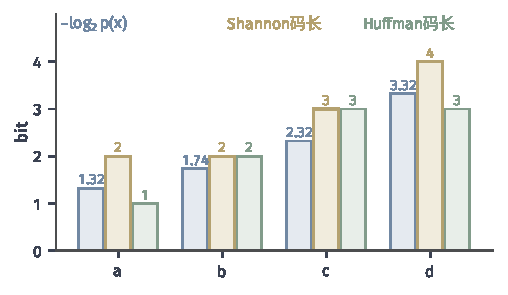
\includegraphics[width=86mm]{figures/07-probability/05-source-coding/matplotlib/lossless-length-vs-selfinfo/figure.pdf}
 \caption{贯穿例中每个符号的自信息$-\log_2p(x)$（蓝）、Shannon码长$\lceil-\log_2p(x)\rceil$（黄）和第~\ref{sec:lossless-model}节码表的码长（绿）。Shannon码长总不小于自信息；后一张码表中$a$与$d$的码长小于自信息，平均码长$1.9$却仍不小于熵$1.846$。}
 \label{fig:lossless-length-vs-selfinfo}
\end{BookInlineFigure}

\paragraph{冗余可以接近一位}
上界中的$+1$不能改进成更小的常数。取二元信源$\mathcal{X}=\{0,1\}$，$p(1)=\theta$。任何唯一可译码的码字至少一位，所以平均码长至少为$1$；而熵
\[
 H(\theta)=-\theta\log_2\theta-(1-\theta)\log_2(1-\theta)
\]
在$\theta\to0$时趋于$0$。$\theta=0.1$时$H=0.469$，最优码仍要$1$位，冗余$0.531$；$\theta$越小，冗余越接近$1$。图~\ref{fig:lossless-binary-bounds}画出这一情形。问题在于每个符号至少要花一位：概率极不均匀时，一个符号所含的信息远少于一位，逐符号编码无法用“半位”来记录它。第~\ref{sec:lossless-block-limits}节把多个符号合成一块编码，正是为了把这一位摊到许多符号上。

\begin{BookInlineFigure}
 \centering
 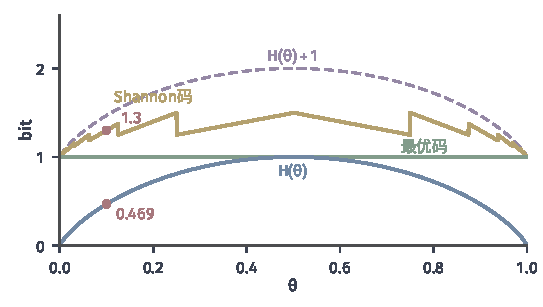
\includegraphics[width=92mm]{figures/07-probability/05-source-coding/matplotlib/lossless-binary-bounds/figure.pdf}
 \caption{二元信源$p(1)=\theta$的逐符号编码。蓝线为熵$H(\theta)$，紫色虚线为上界$H(\theta)+1$，黄线为Shannon码的平均码长，绿线为最优码的平均码长$1$。红点标出$\theta=0.1$处的$H=0.469$与Shannon码长$1.3$。黄线在$\theta=1/2$处另有一个孤立的取值$1$，图中未画出。}
 \label{fig:lossless-binary-bounds}
\end{BookInlineFigure}

\paragraph{确定源}
定理~\ref{thm:lossless-entropy-bound}要求至少两个符号有正概率。若只有一个符号$x_0$，$p(x_0)=1$，则$H(X)=0$，式~\eqref{eq:lossless-shannon-length}给出的码长是$0$，即空码字。这时要看解码器知道什么。

若消息长度$n$事先约定，接收方知道消息必定是$x_0x_0\cdots x_0$（$n$个），什么都不必发送，平均码长为$0$，等于熵。若长度没有约定，空码字无法告诉接收方发出了几个符号：$n=1$和$n=5$的消息都编成空串。由第~\ref{sec:lossless-decodability}节，唯一可译码不含空码字，每个符号至少一位，平均码长至少为$1$；另一种做法是单独传送长度$n$，所需位数随$n$增长，但这已不是逐符号编码的问题。所以确定源的“零码长”只在长度已知时成立，这正是定理把它排除在外的原因。


\section{编码方法}
\label{sec:lossless-methods}

前两节确定了标准：解码必须唯一，评价看平均码长，下界是熵。Shannon码满足上界，却可能比简单的码还差。本节构造两种实际使用的编码。Huffman编码针对给定的有限符号表，直接求出平均码长最短的前缀码；算术编码不给单个符号分配码字，而是把整条消息对应到$[0,1)$中的一个小区间。两者处理的对象不同，比较时要统一被编码的对象和消息的终止规则。

\subsection{Huffman编码}
\label{sec:lossless-huffman}

在所有二进制前缀码中，哪一个的平均码长最小？前缀码只有有限多种“有用的”码长组合，原则上可以穷举，但符号多时组合数巨大。\term{Huffman编码}（Huffman coding）给出一个只需反复合并的构造\scite{vision-huffman1952}。

\paragraph{主要思想}
从码树的角度看，平均码长是各叶结点深度按概率加权的和。概率小的符号应当放在深处，而最深处的两片叶子一定是兄弟。把这两片叶子合并成它们的父结点，问题就变成一个少一个符号的同类问题。Huffman编码的做法是：每次把概率最小的两个符号合并成一个新符号，新符号的概率是两者之和，直到只剩一个符号；再沿合并的过程从根往下分配$0$和$1$。

要说明这样做是最优的，需要两步：先证明存在一个最优码，其中概率最小的两个符号恰好是最深处的一对兄弟；再证明合并之后的问题与原问题的最优值只相差一个常数。

称前缀码$c^{\star}$为最优的，如果它的平均码长在所有前缀码中最小。最优码存在：任取一个前缀码$c_0$，平均码长不超过$L(c_0)$的前缀码满足
\[
 \ell(x)\leq\frac{L(c_0)}{\min_y p(y)}\quad\text{对每个}x ,
\]
只有有限多种码长组合，其中必有平均码长最小的一个。

\begin{lemma}[最优码的结构]
\label{lem:lossless-optimal-structure}
设$\lvert\mathcal{X}\rvert\geq2$，各$p(x)>0$，$u,v$是概率最小的两个符号（有并列时任取）。则存在最优前缀码$c^{\star}$，使得：
\begin{enumerate}
 \item 若$p(x)>p(y)$，则$\ell(x)\leq\ell(y)$；
 \item $c^{\star}(u)$与$c^{\star}(v)$长度相同且为最大码长，两者只有最后一位不同。
\end{enumerate}
\end{lemma}

\begin{proof}
第一条对每个最优码都成立。若$p(x)>p(y)$而$\ell(x)>\ell(y)$，交换$x,y$的码字，得到的仍是前缀码，平均码长的变化为
\[
 \begin{aligned}
 &p(x)\ell(y)+p(y)\ell(x)-p(x)\ell(x)-p(y)\ell(y)\\
 &\qquad=-\bigl(p(x)-p(y)\bigr)\bigl(\ell(x)-\ell(y)\bigr)<0 ,
 \end{aligned}
\]
与最优性矛盾。

其次，在任一最优码中，设$s$是一个最长的码字，把$s$的最后一位取反得到串$s'$，称为$s$的兄弟。$s'$一定是码字。否则，任何以$s'$开头的码字长度都不小于$\lvert s\rvert$，而$s$已是最长，于是没有码字以$s'$开头；这时删去$s$的最后一位，得到的码仍是前缀码，平均码长减少$p(\cdot)>0$，矛盾。所以最长码字成对出现，每对是兄弟。

最后，取一对最长的兄弟码字，设它们属于符号$y,y'$。把$u$与$y$的码字交换，再把$v$与$y'$的码字交换（若$u$或$v$本来就是$y$或$y'$，相应的交换省去）。由于$p(u)\leq p(y)$而$\ell(u)\leq\ell(y)$（$y$的码长是最大码长），按上面的计算，这一交换使平均码长的变化为
\[
 \bigl(p(y)-p(u)\bigr)\bigl(\ell(u)-\ell(y)\bigr)\leq0 ,
\]
第二次交换同理。交换后的码平均码长不增，仍是最优码，且$u,v$占据最深的一对兄弟。第一条对它仍成立。
\end{proof}

图~\ref{fig:lossless-huffman-exchange}用贯穿例演示交换。码树的深度固定为$1,2,3,3$，若把概率最大的$a$放在深度$3$、概率最小的$d$放在深度$1$，平均码长为$2.5$；交换两者后，平均码长减少
\[
 (0.4-0.1)\times(3-1)=0.6 ,
\]
变为$1.9$。

\begin{BookInlineFigure}
 \centering
 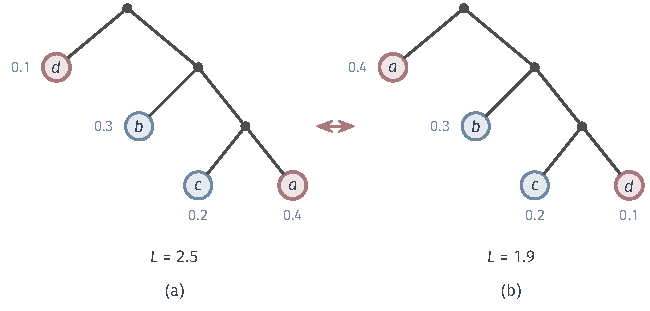
\includegraphics[width=110mm]{figures/07-probability/05-source-coding/tikz/lossless-huffman-exchange/figure.pdf}
 \caption{交换论证。两棵码树形状相同，叶结点旁为概率。(a)把概率$0.4$的$a$放在深度$3$、概率$0.1$的$d$放在深度$1$，平均码长$2.5$。(b)交换两片红色叶子后平均码长降为$1.9$。}
 \label{fig:lossless-huffman-exchange}
\end{BookInlineFigure}

接下来比较合并前后的问题。设$u,v$如引理所述，构造缩减的字母表$\mathcal{X}'$：去掉$u,v$，加入一个新符号$z$，其概率为$p'(z)=p(u)+p(v)$，其余符号概率不变。给定$\mathcal{X}'$上的前缀码$c'$，令
\[
 c(u)=c'(z)0,\qquad c(v)=c'(z)1,\qquad c(x)=c'(x)\ (x\neq u,v),
\]
即把叶子$z$展开成两片兄弟叶子。$c$仍是前缀码，平均码长满足
\begin{equation}
 L(c)=L(c')+p(u)+p(v) ,
 \label{eq:lossless-huffman-reduction}
\end{equation}
因为只有$u,v$的码长比$z$多一位。反过来，若$\mathcal{X}$上的前缀码中$u,v$是兄弟叶子，把它们合并成父结点就得到$\mathcal{X}'$上的前缀码，平均码长的关系同样是式~\eqref{eq:lossless-huffman-reduction}。

\begin{theorem}[Huffman编码的最优性]
\label{thm:lossless-huffman-optimal}
设$\mathcal{X}$有限，$\lvert\mathcal{X}\rvert\geq2$，各$p(x)>0$。Huffman编码的平均码长在所有二进制唯一可译码中最小。
\end{theorem}

\begin{proof}
由Kraft–McMillan不等式，唯一可译码能实现的码长都能由前缀码实现，所以只需与前缀码比较。对符号个数$m=\lvert\mathcal{X}\rvert$作归纳。$m=2$时Huffman编码给出码字$0,1$，平均码长为$1$；唯一可译码不含空码字，平均码长至少为$1$，结论成立。

设结论对$m-1$个符号成立。Huffman编码先合并概率最小的$u,v$，在缩减字母表$\mathcal{X}'$上得到Huffman码$h'$，再把$z$展开，得到$\mathcal{X}$上的码$h$。由式~\eqref{eq:lossless-huffman-reduction}，
\[
 L(h)=L(h')+p(u)+p(v).
\]
取引理~\ref{lem:lossless-optimal-structure}给出的最优码$c^{\star}$，其中$u,v$是兄弟叶子，合并得到$\mathcal{X}'$上的前缀码$c'$，同样有
\[
 L(c^{\star})=L(c')+p(u)+p(v).
\]
由归纳假设，$h'$在$\mathcal{X}'$上最优，$L(h')\leq L(c')$。两式相减得$L(h)\leq L(c^{\star})$，所以$h$也是最优码。
\end{proof}

式~\eqref{eq:lossless-huffman-reduction}还给出一个算平均码长的捷径：每合并一次，平均码长增加被合并两项的概率之和。所以Huffman码的平均码长等于各次合并所得新结点的概率之和。

\paragraph{计算过程}
下面在贯穿例$p=(0.4,0.3,0.2,0.1)$上逐步执行。

\needspace{6\baselineskip}
\paragraph{变量}
\begin{itemize}
 \item 待合并结点的集合$\mathcal{Q}$：每个结点是一棵子树，带有权重，即子树中所有叶结点的概率之和。实现时用按权重排序的优先队列。
 \item 子树内部的连接：每个内部结点记住它的两个子结点，以及分别通向它们的边上的位$0$或$1$。
 \item 并列规则：权重相同时，先进入$\mathcal{Q}$的结点先取出。原始符号在初始化时进入，合并产生的结点后进入。
\end{itemize}

\paragraph{初始化}
每个符号是一个只有一片叶子的子树，权重为它的概率，全部放入$\mathcal{Q}$。例中
\[
 \mathcal{Q}=\{a:0.4,\ b:0.3,\ c:0.2,\ d:0.1\}.
\]

\needspace{6\baselineskip}
\paragraph{每轮更新}
当$\mathcal{Q}$中多于一个结点时：
\begin{enumerate}
 \item \textbf{取出两个最小权重。}从$\mathcal{Q}$中依次取出权重最小的结点$s_1$与次小的结点$s_2$。例中第一轮取出$d$（$0.1$）与$c$（$0.2$）。
 \item \textbf{合并。}新建内部结点$t$，以$s_1,s_2$为子结点，通向$s_1$的边记$0$，通向$s_2$的边记$1$，权重为两者之和。例中第一轮
 \[
  t_1=\{d,c\},\qquad 0.1+0.2=0.3 .
 \]
 \item \textbf{放回。}把$t$放入$\mathcal{Q}$。例中第一轮后
 \[
  \mathcal{Q}=\{a:0.4,\ b:0.3,\ t_1:0.3\}.
 \]
\end{enumerate}
例中第二轮，$b$与$t_1$的权重都是$0.3$，按并列规则先取出$b$，再取出$t_1$，合并为权重$0.6$的结点$t_2$，$b$一侧记$0$，$t_1$一侧记$1$：
\[
 \mathcal{Q}=\{a:0.4,\ t_2:0.6\}.
\]
第三轮取出$a$与$t_2$，合并为权重$1$的根结点$t_3$，$a$一侧记$0$，$t_2$一侧记$1$，$\mathcal{Q}$中只剩一个结点，合并结束。图~\ref{fig:lossless-huffman-steps}画出各轮之后的森林。

\begin{BookInlineFigure}
 \centering
 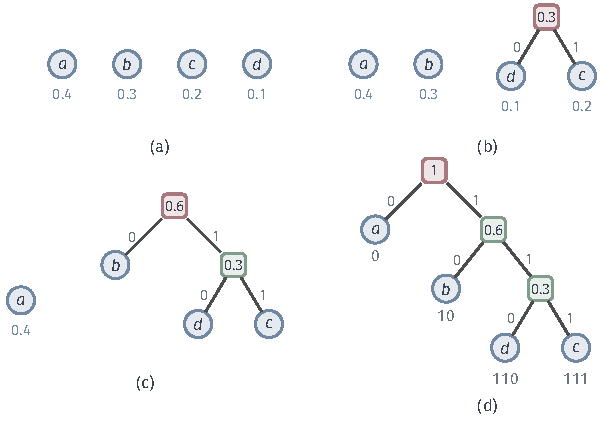
\includegraphics[width=102mm]{figures/07-probability/05-source-coding/tikz/lossless-huffman-steps/figure.pdf}
 \caption{贯穿例的Huffman合并。蓝圈为原始符号及其概率，方框为合并产生的结点及其权重，红框是该轮新产生的结点，边旁为分配的位。(a)初始；(b)合并$d,c$；(c)合并$b$与$\{d,c\}$；(d)合并$a$得到根，叶结点下方为码字。}
 \label{fig:lossless-huffman-steps}
\end{BookInlineFigure}

\paragraph{读出码字}
从根出发走到每片叶子，依次写下经过的位，就是该符号的码字。例中
\[
 a\mapsto0,\qquad b\mapsto10,\qquad d\mapsto110,\qquad c\mapsto111 .
\]
码长为$1,2,3,3$。按合并新结点的权重求和，
\[
 L=0.3+0.6+1.0=1.9 ,
\]
与按定义逐项计算一致。最终得到的码长与第~\ref{sec:lossless-model}节的码表相同，只是$c,d$的码字互换；两者长度相同，平均码长都是$1.9$，冗余为$1.9-1.846=0.054$。由定理~\ref{thm:lossless-huffman-optimal}，在这个概率表下没有平均码长小于$1.9$的唯一可译码。

\paragraph{算法分析}
用二叉堆实现优先队列时，每轮取出两次、放入一次，各需$O(\log m)$次比较，共$m-1$轮，总计算量为$O(m\log m)$；若概率已经排好序，可以用两个先进先出队列在$O(m)$时间内完成。并列规则不同时，得到的码树和码长都可能不同，但由定理~\ref{thm:lossless-huffman-optimal}，平均码长相同。最长码字可以长达$m-1$位，例如概率按$1/2,1/4,1/8,\dots$递减时码树退化成一条链。

最优性的范围要说清楚。定理只断言：对一个给定的有限字母表和给定的概率表，在逐符号的二进制唯一可译码中，Huffman码平均码长最短。它不说明每个符号至少要花这么多位；若把若干符号合成一块再编码，被编码的字母表就换成了$\mathcal{X}^n$，有$\lvert\mathcal{X}\rvert^n$个“符号”，Huffman码要对这个大字母表重新构造，平均到每个原始符号上可以更短（第~\ref{sec:lossless-block-limits}节）。代价是码表规模随块长指数增长。

\subsection{算术编码}
\label{sec:lossless-arithmetic}

Huffman码给每个符号整数位，概率极不均匀时，一个符号可能只含零点几位信息，却至少要花一位。另一条路是不给符号分配码字，而给整条消息分配码字。\term{算术编码}（arithmetic coding）用一个逐步缩小的区间来做这件事\scite{math-witten1987arithmetic}。

\paragraph{主要思想}
把$[0,1)$看成单位质量，按概率分给各个符号：贯穿例中$a$占$[0,0.4)$，$b$占$[0.4,0.7)$，$c$占$[0.7,0.9)$，$d$占$[0.9,1)$。读到第一个符号，就留下它的那一段；在这一段里再按同样的比例分给四个符号，读到第二个符号再留下相应的一小段；如此继续。读完整条消息时剩下的区间，长度恰好是这条消息的概率。

用公式写出来。给$\mathcal{X}$中的符号排定顺序，记累积概率
\[
 F(x)=\sum_{y\prec x}p(y),
\]
其中$y\prec x$表示$y$排在$x$之前。贯穿例按$a,b,c,d$排序，$F(a)=0$，$F(b)=0.4$，$F(c)=0.7$，$F(d)=0.9$。消息$x_{1:n}$对应的区间$[\mathrm{lo}_k,\mathrm{lo}_k+w_k)$按下式逐步更新：
\begin{equation}
 \mathrm{lo}_0=0,\quad w_0=1;\qquad
 \mathrm{lo}_k=\mathrm{lo}_{k-1}+w_{k-1}F(x_k),\quad w_k=w_{k-1}\,p(x_k).
 \label{eq:lossless-arith-update}
\end{equation}
第$k$步把当前区间按比例切开，留下第$k$个符号的那一份。由此$w_n=\prod_{k}p(x_k)$，按式~\eqref{eq:lossless-product}正是$p(x_{1:n})$。记$J(x_{1:n})=[\mathrm{lo}_n,\mathrm{lo}_n+w_n)$。

固定消息长度$n$，所有长度为$n$的消息的区间$J(x_{1:n})$两两不交，并且铺满$[0,1)$。对$n$归纳：$n=0$时只有$[0,1)$；长度为$k$的消息的区间由长度为$k-1$的前缀的区间按概率切成$\lvert\mathcal{X}\rvert$份得到，各份不交且铺满原区间。

剩下的问题是怎样用尽量少的位说出“消息的区间是哪一个”。办法与Kraft不等式的证明相同：找一个完全落在$J(x_{1:n})$内的二进区间，发送它对应的二进制串。取
\begin{equation}
 \ell=\Bigl\lceil\log_2\frac{1}{w_n}\Bigr\rceil+1,\qquad
 k=\bigl\lceil\mathrm{lo}_n2^{\ell}\bigr\rceil ,
 \label{eq:lossless-arith-codeword}
\end{equation}
码字是整数$k$的$\ell$位二进制表示（不足$\ell$位时前面补$0$），它对应二进区间$[k2^{-\ell},(k+1)2^{-\ell})$。

这个二进区间落在$J(x_{1:n})$内。左端：$k\geq\mathrm{lo}_n2^{\ell}$，所以$k2^{-\ell}\geq\mathrm{lo}_n$。右端：$k<\mathrm{lo}_n2^{\ell}+1$，再由$\ell$的取法$2^{-\ell}\leq w_n/2$，于是
\[
 (k+1)2^{-\ell}<\mathrm{lo}_n+2\cdot2^{-\ell}\leq\mathrm{lo}_n+w_n .
\]
同一长度的不同消息区间不交，它们的二进区间也不交，所以这些码字中没有一个是另一个的前缀：对固定的$n$，算术编码是$\mathcal{X}^n$上的前缀码。码长满足
\begin{equation}
 \ell<\log_2\frac{1}{p(x_{1:n})}+2 ,
 \label{eq:lossless-arith-length}
\end{equation}
对消息取期望，平均码长小于$nH(X)+2$，每符号小于$H(X)+2/n$。消息越长，这额外的两位摊得越薄。

解码是同一过程的逆向。设收到码字，算出$v=k2^{-\ell}$，它落在$J(x_{1:n})$中。第一个符号是唯一满足$F(x)\leq v<F(x)+p(x)$的$x$；把$v$换成$(v-F(x_1))/p(x_1)$，即在留下的子区间中重新标定到$[0,1)$，再按同样的规则读出第二个符号，如此重复$n$次。解码器必须使用与编码器完全相同的符号顺序和概率。

\paragraph{计算过程}
下面用贯穿例对消息$abac$逐步演示，$n=4$事先约定。

\needspace{6\baselineskip}
\paragraph{变量}
\begin{itemize}
 \item 概率表$p(x)$与累积概率表$F(x)$：各$\lvert\mathcal{X}\rvert$个数，编码器与解码器共享。
 \item $\mathrm{lo}$：当前区间的左端点。
 \item $w$：当前区间的长度。
 \item 消息长度$n$：事先约定，或按下文的终止规则处理。
\end{itemize}

\paragraph{初始化}
$\mathrm{lo}=0$，$w=1$。例中$F=(0,0.4,0.7,0.9)$，$p=(0.4,0.3,0.2,0.1)$。

\needspace{6\baselineskip}
\paragraph{每轮更新}
对$k=1,\dots,n$，读入符号$x_k$：
\begin{enumerate}
 \item \textbf{移左端。}按式~\eqref{eq:lossless-arith-update}，$\mathrm{lo}\leftarrow\mathrm{lo}+w\,F(x_k)$。
 \item \textbf{缩长度。}$w\leftarrow w\,p(x_k)$。
\end{enumerate}
例中四轮的结果如下（先算左端，再用旧的$w$乘概率）：
\[
 \begin{aligned}
 &a:&\mathrm{lo}&=0+1\times0=0, & w&=1\times0.4=0.4,\\
 &b:&\mathrm{lo}&=0+0.4\times0.4=0.16, & w&=0.4\times0.3=0.12,\\
 &a:&\mathrm{lo}&=0.16+0.12\times0=0.16, & w&=0.12\times0.4=0.048,\\
 &c:&\mathrm{lo}&=0.16+0.048\times0.7=0.1936, & w&=0.048\times0.2=0.0096.
 \end{aligned}
\]
读完$n$个符号后结束，最终区间为
\[
 J(abac)=[0.1936,\,0.2032),\qquad w_4=0.0096=p(abac).
\]

\paragraph{输出码字}
由式~\eqref{eq:lossless-arith-codeword}，
\[
 \ell=\lceil6.703\rceil+1=8,\qquad k=\lceil0.1936\times256\rceil=\lceil49.56\rceil=50 ,
\]
码字是$50$的$8$位二进制表示$00110010$，对应二进区间
\[
 [50/256,\,51/256)=[0.1953,\,0.1992)\subset[0.1936,\,0.2032).
\]
图~\ref{fig:lossless-arith-intervals}逐行画出区间的缩小过程。这条消息的自信息是$\log_2(1/0.0096)=6.703$位，算术编码用了$8$位，比上一小节的Huffman码字串$0\,10\,0\,111$多一位。对这样短的消息，式~\eqref{eq:lossless-arith-length}中的两位额外开销相当可观；它的好处要在长消息中才显现。

\begin{BookInlineFigure}
 \centering
 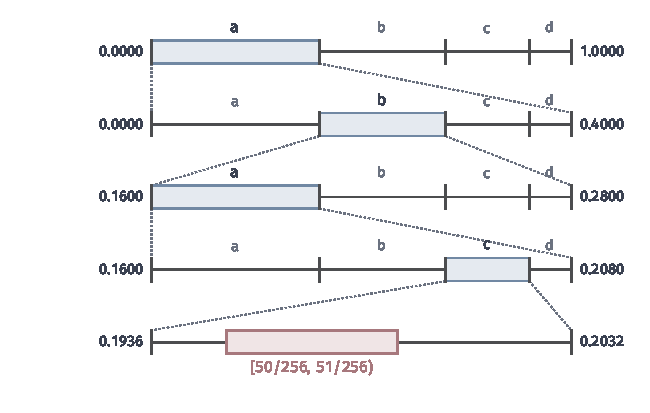
\includegraphics[width=110mm]{figures/07-probability/05-source-coding/matplotlib/lossless-arith-intervals/figure.pdf}
 \caption{算术编码消息$abac$。每一行把当前区间放大到同样宽度，两侧数字为区间端点，按$4:3:2:1$切给$a,b,c,d$；浅蓝格是读到的符号留下的子区间，虚线把它放大到下一行。最后一行是最终区间$[0.1936,0.2032)$，红框是码字$00110010$对应的二进区间。}
 \label{fig:lossless-arith-intervals}
\end{BookInlineFigure}

同样长度的另一条消息$abad$只在最后一步不同：$\mathrm{lo}=0.16+0.048\times0.9=0.2032$，$w=0.0048$，于是$\ell=\lceil7.703\rceil+1=9$，$k=\lceil0.2032\times512\rceil=105$，码字为$001101001$。它与$00110010$在第$6$位就不同，谁也不是谁的前缀，这正是两条消息的区间$[0.1936,0.2032)$与$[0.2032,0.2080)$不交的结果。

\paragraph{解码}
解码器收到$00110010$，得$v=50/256=0.1953$，逐步读出：
\[
 \begin{aligned}
 &v=0.1953\in[0,0.4) &&\Rightarrow a, & v&\leftarrow0.1953/0.4=0.4883,\\
 &v=0.4883\in[0.4,0.7) &&\Rightarrow b, & v&\leftarrow(0.4883-0.4)/0.3=0.2943,\\
 &v=0.2943\in[0,0.4) &&\Rightarrow a, & v&\leftarrow0.2943/0.4=0.7357,\\
 &v=0.7357\in[0.7,0.9) &&\Rightarrow c .
 \end{aligned}
\]
读满$n=4$个符号后停止，恢复出$abac$。

\paragraph{终止规则}
上面的码对固定的$n$是前缀码，不同长度的消息之间却可能冲突：同一个码字所在的二进区间，既落在某条长度为$4$的消息的区间里，也落在它的前缀$aba$的区间里。所以接收方必须知道消息在哪里结束。常用两种约定。一是事先约定或单独传送长度$n$；单独传送时，用一个整数的前缀码，大约需要$2\log_2n$位。二是在字母表中加入终止符号，给它一个小概率$\varepsilon$，其余符号的概率乘以$1-\varepsilon$；消息总以终止符号结束，于是“消息加终止符”组成的集合中没有一条是另一条的前缀。终止符号的代价是消息末尾多出$\log_2(1/\varepsilon)$位，每个普通符号多出$\log_2(1/(1-\varepsilon))$位。

\paragraph{有限精度}
上面的计算用的是精确实数，消息长时$w$小到无法用浮点数表示。实际实现用整数：概率表写成整数频数$f(x)$，总和为$T$；区间端点用$B$位整数表示。每读一个符号，按频数比例切分整数区间并向下取整。每当区间整个落在$[0,1/2)$或$[1/2,1)$中，最高位已经确定，立即输出这一位，并把区间放大一倍，使区间长度保持在一个固定范围内；区间跨越中点但很窄时，记下“待定位”的个数，等以后确定方向再一并输出。

整数实现能正确解码的关键，是编码器与解码器做完全相同的整数运算和取整：只要两边一致，取整只是把每个子区间的长度稍微改动，改动后的子区间仍两两不交、铺满当前区间。取整的代价是码长比式~\eqref{eq:lossless-arith-length}稍长，$B$足够大时这个损失很小。此外每个可能出现的符号都需要$f(x)\geq1$，否则它的子区间长度为零，无法编码。

\paragraph{模型与实际概率}
编码器和解码器用的概率表$q$称为模型，它可以与信源的真实分布$p$不同。只要两边用同一个$q$，并且消息中出现的每个符号都有$q(x)>0$，上面的论证不变，只需把$p$换成$q$：码长满足
\[
 \ell<\log_2\frac{1}{q(x_{1:n})}+2 ,
\]
解码仍然正确。模型不准只让码长变长，对独立同分布消息，平均每符号码长约为$H(X)+D_{\mathrm{KL}}(p\Vert q)$，第~\ref{sec:lossless-finite-resources}节将给出这一点的精确界。

若模型给一个实际出现的符号零概率，$q(x_k)=0$，则$w$在这一步变成$0$，区间消失，这条消息无法编码。这不是“码长变长”的问题，而是编码本身无法继续。所以模型必须给每个可能出现的符号留下正概率。

模型也可以随已读的符号改变，只要编码器和解码器按同一规则更新：把式~\eqref{eq:lossless-arith-update}中的$p(x_k)$与$F(x_k)$换成依赖于$x_{1:k-1}$的条件概率与累积概率，区间长度就变成这些条件概率的乘积，上面的论证照样成立。这使算术编码可以配合任意按顺序给出概率的模型，而Huffman码要求事先给定一个固定的概率表。

\paragraph{与Huffman编码比较}
比较两种方法时，必须让它们编码同一个对象，按同一个终止规则。Huffman码是逐符号的前缀码，消息结束靠约定长度或额外的码字；按长度为$n$的整条消息计算，它的平均码长为$n\times1.9$，每符号$1.9$位。算术编码在$n$已知时，每符号平均码长小于
\[
 H(X)+\frac{2}{n}=1.846+\frac{2}{n} ,
\]
$n=4$时这个上界是$2.346$，比Huffman码差；$n=40$时为$1.896$，已低于Huffman码。

图~\ref{fig:lossless-arith-length}在一条长$400$的随机消息上验证这些数值。用真实模型$p$编码时，每符号码长从短消息时的约$3$位逐步降到$1.855$位，接近熵$1.846$；用均匀模型$q(x)=1/4$编码时，码长恰为$2n+1$，每符号趋于$2$，即$H+D_{\mathrm{KL}}(p\Vert q)=1.846+0.154$。右图显示，在每个前缀长度上，码长与自信息之差都落在$[1,2)$中，这正是式~\eqref{eq:lossless-arith-codeword}的取整与$+1$造成的。

\begin{BookInlineFigure}
 \centering
 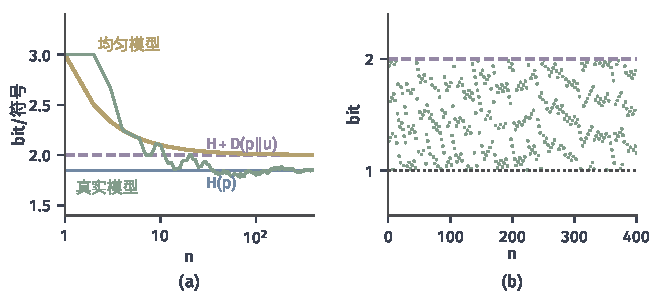
\includegraphics[width=110mm]{figures/07-probability/05-source-coding/matplotlib/lossless-arith-length/figure.pdf}
 \caption{一条由贯穿例信源独立生成、长$400$的消息（随机种子$7$）。(a)各前缀长度$n$下算术编码的每符号码长，横轴为对数坐标：绿线用真实模型，黄线用均匀模型；蓝线为熵$H=1.846$，紫色虚线为$H+D_{\mathrm{KL}}(p\Vert u)=2$。(b)真实模型下码长与消息自信息之差，所有点落在$[1,2)$中。}
 \label{fig:lossless-arith-length}
\end{BookInlineFigure}


\section{块编码的压缩极限}
\label{sec:lossless-block-limits}

逐符号编码的冗余可以接近一位，原因是每个符号至少花一位。把$n$个符号合成一块编码，可以从两个方向利用这一点。一是仍要求每块精确还原，但让整数码长的取整损失摊到$n$个符号上；二是放弃对极少数块的还原，只给高概率的块编号，从而使用固定长度的码字。两条路都把每符号所需的位数压到熵$H(X)$，但允许的码长形式和错误要求不同。本节设$X_1,X_2,\dots$独立同分布，服从字母表$\mathcal{X}$上的$p$。

\subsection{零错误的变长块编码}
\label{sec:lossless-variable-block}

把块$x_{1:n}$看作字母表$\mathcal{X}^n$中的一个符号，它的概率由式~\eqref{eq:lossless-product}给出。对这个大字母表直接应用定理~\ref{thm:lossless-entropy-bound}，需要知道块的熵。

\begin{lemma}[独立块的熵]
\label{lem:lossless-block-entropy}
若$X_1,\dots,X_n$独立同分布，则
\begin{equation}
 H(X_{1:n})=nH(X_1).
 \label{eq:lossless-block-entropy}
\end{equation}
\end{lemma}

\begin{proof}
由式~\eqref{eq:lossless-product}，块的自信息是各符号自信息之和：
\[
 -\log_2p(x_{1:n})=\sum_{i=1}^{n}\bigl(-\log_2p(x_i)\bigr).
\]
在$x_{1:n}$处取值为$X_{1:n}$，两边取期望，由期望的线性性与同分布，
\[
 \begin{aligned}
 H(X_{1:n})&=\mathbb{E}\Bigl[\sum_{i=1}^{n}-\log_2p(X_i)\Bigr]\\
 &=\sum_{i=1}^{n}H(X_i)=nH(X_1). \qedhere
 \end{aligned}
\]
\end{proof}

\begin{theorem}[变长块编码]
\label{thm:lossless-variable-block}
设$\lvert\mathcal{X}\rvert\geq2$，各$p(x)>0$，块长$n\geq1$。$\mathcal{X}^n$上平均码长最短的唯一可译码$c_n^{\star}$满足
\begin{equation}
 H(X)\leq\frac{L(c_n^{\star})}{n}<H(X)+\frac1n .
 \label{eq:lossless-block-bound}
\end{equation}
\end{theorem}

\begin{proof}
$\mathcal{X}^n$至少有两个元素，每个块的概率都是正的。对字母表$\mathcal{X}^n$与块的分布应用定理~\ref{thm:lossless-entropy-bound}，任何唯一可译码的平均码长不小于$H(X_{1:n})$，而按块的自信息取整的Shannon码平均码长小于$H(X_{1:n})+1$。最优码介于两者之间：
\[
 H(X_{1:n})\leq L(c_n^{\star})<H(X_{1:n})+1 .
\]
由式~\eqref{eq:lossless-block-entropy}代入$H(X_{1:n})=nH(X)$，再除以$n$即得。
\end{proof}

最优码$c_n^{\star}$可以用Huffman编码对$\lvert\mathcal{X}\rvert^n$个块求出。整数码长带来的不到一位的冗余是每块一次，摊到每个符号上不足$1/n$位。对确定源，第~\ref{sec:lossless-average-length}节的讨论照样适用：长度已知时什么都不必发送；长度未约定时，空码字无法区分块数。

\paragraph{贯穿例}
对贯穿例的$n=1,\dots,6$分别构造块上的Huffman码，每符号平均码长为
\[
 \begin{gathered}
 1.900,\quad 1.865,\quad 1.859,\\
 1.853,\quad 1.853,\quad 1.851 ,
 \end{gathered}
\]
都在$[1.846,\,1.846+1/n)$中。图~\ref{fig:lossless-block-huffman}(a)把它们与块上Shannon码的每符号平均码长一起画出。数列不一定单调：$n=5$的值$1.85347$略大于$n=4$的值$1.85323$。定理只保证上界$H+1/n$单调下降，最优冗余本身随块长的变化取决于块概率怎样与$2$的整数次幂对齐。

\begin{BookInlineFigure}
 \centering
 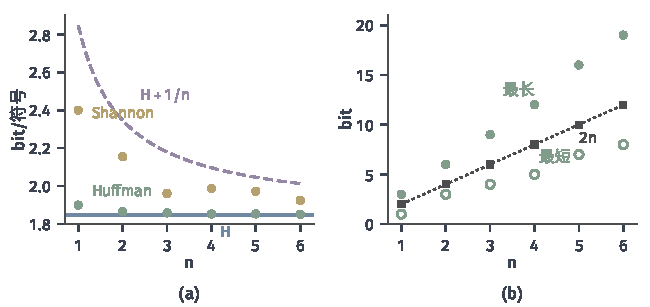
\includegraphics[width=110mm]{figures/07-probability/05-source-coding/matplotlib/lossless-block-huffman/figure.pdf}
 \caption{贯穿例的变长块编码，块长$n=1,\dots,6$。(a)每符号平均码长：绿点为块上的Huffman码，黄点为块上的Shannon码，蓝线为熵$H=1.846$，紫色虚线为上界$H+1/n$。(b)块上Huffman码的最短码字（空心绿点）与最长码字（实心绿点），灰色方点为同一块长的定长码$2n$位。}
 \label{fig:lossless-block-huffman}
\end{BookInlineFigure}

块编码对概率很不均匀的信源收益更大。第~\ref{sec:lossless-average-length}节的二元信源$\theta=0.1$，熵为$0.469$，逐符号编码至少要$1$位。块上Huffman码的每符号平均码长在$n=1,\dots,6$时为
\[
 \begin{gathered}
 1.000,\quad 0.645,\quad 0.533,\\
 0.493,\quad 0.480,\quad 0.470 ,
 \end{gathered}
\]
$n=6$时已与熵只差$0.001$位；$n=7$时反而回升到$0.474$。逐符号编码一半以上的位数是取整造成的，合成块以后这部分几乎全部收回。

\paragraph{平均保证不管最坏情形}
式~\eqref{eq:lossless-block-bound}是关于平均的。图~\ref{fig:lossless-block-huffman}(b)显示，块上Huffman码的最长码字随$n$增长得比定长码快：$n=6$时最长码字$19$位，而定长码只需$12$位；最长码字属于$dddddd$这样概率为$10^{-6}$的块。零错误的要求意味着这些罕见的块也必须有码字，它们只能放在码树的深处。

块编码的另外两项代价不在式~\eqref{eq:lossless-block-bound}中。一是码本：块上的码表有$4^n$项，$n=6$时为$4096$项，编码器与解码器都要存储，若码表要随消息一起传送，还要计入它的描述长度。二是构造与查找：Huffman构造需要$O(4^n\cdot n)$次比较。所以“块越长越接近熵”只在不计码本与计算代价时成立，第~\ref{sec:lossless-finite-resources}节把这些代价放在一起比较。

\subsection{允许错误的定长块编码}
\label{sec:lossless-fixed-block}

现在换一种要求：码字都等长，每块用同样多的位，但允许极少数块无法还原。这时问题变成“需要给多少个块编号”。四符号信源长度为$n$的块共有$4^n$个，全部编号需要$2n$位；如果绝大部分概率集中在少得多的块上，只给这些块编号就够了。

\begin{definition}[定长块编码与码率]
\label{def:lossless-fixed-length}
块长为$n$、含$M_n$个码字的定长块编码由编码映射$f_n:\mathcal{X}^n\to\{1,\dots,M_n\}$与解码映射$g_n:\{1,\dots,M_n\}\to\mathcal{X}^n$组成。每个编号用$\lceil\log_2M_n\rceil$位表示，\term{码率}（code rate）定义为
\begin{equation}
 R_n=\frac{\log_2M_n}{n}
 \label{eq:lossless-rate}
\end{equation}
单位是bit每源符号。错误概率为
\begin{equation}
 P_{\mathrm{e}}^{(n)}=\mathbb{P}\bigl(g_n(f_n(X_{1:n}))\neq X_{1:n}\bigr).
 \label{eq:lossless-error-prob}
\end{equation}
\end{definition}

\paragraph{自信息的集中}
要找出“概率集中在哪些块上”，先看一个块的每符号自信息$-\frac1n\log_2p(X_{1:n})$。由引理~\ref{lem:lossless-block-entropy}的证明，它是$n$个独立同分布随机变量
\[
 Y_i=-\log_2p(X_i)
\]
的样本平均。$Y_i$只取有限个值，均值是$H(X)$，方差
\[
 \sigma^2=\operatorname{Var}(Y_1)=\sum_xp(x)\bigl(-\log_2p(x)-H(X)\bigr)^2
\]
有限。第~\ref{chap:laws-of-large-numbers}章的弱大数律于是给出下面的结论。

\begin{theorem}[渐近均分性]
\label{thm:lossless-aep}
设$X_1,X_2,\dots$独立同分布，取值于有限字母表，各$p(x)>0$。则对每个$\varepsilon>0$，
\begin{equation}
 \mathbb{P}\Bigl(\Bigl\lvert-\frac1n\log_2p(X_{1:n})-H(X)\Bigr\rvert\geq\varepsilon\Bigr)\leq\frac{\sigma^2}{n\varepsilon^2}\xrightarrow[n\to\infty]{}0 .
 \label{eq:lossless-aep}
\end{equation}
\end{theorem}

\begin{proof}
$-\frac1n\log_2p(X_{1:n})=\frac1n\sum_iY_i$，其期望为$H(X)$，方差为$\sigma^2/n$。对它用第~\ref{chap:tail-probabilities}章的Chebyshev不等式即得。
\end{proof}

这一性质称为\term{渐近均分性}（asymptotic equipartition property）。名称的含义是：$n$大时，实际出现的块几乎都满足
\[
 p(x_{1:n})\approx2^{-nH(X)},
\]
即它们的概率“近似相等”，都在$2^{-n(H\pm\varepsilon)}$之间。这并不是说最可能的块概率接近$2^{-nH}$：贯穿例中最可能的块$aa\cdots a$的概率是$0.4^n=2^{-1.32n}$，远大于$2^{-1.85n}$；只是这样的块太少，合起来的概率可以忽略。

图~\ref{fig:lossless-aep-concentration}画出贯穿例中每符号自信息的精确分布。它按块中$a,b,c,d$的个数枚举所有类型，逐类求和得到，没有用到模拟。$n=10$时分布还很宽，落在$H\pm0.1$内的概率只有$0.337$；$n=250$时，这一概率升到$0.990$。

\begin{BookInlineFigure}
 \centering
 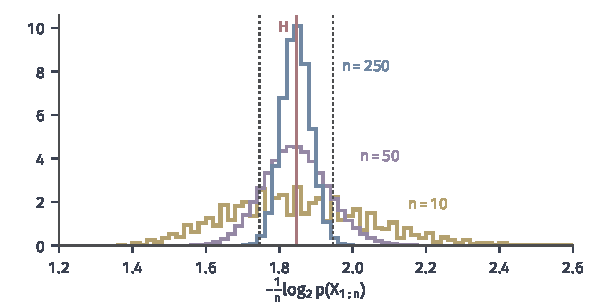
\includegraphics[width=100mm]{figures/07-probability/05-source-coding/matplotlib/lossless-aep-concentration/figure.pdf}
 \caption{贯穿例中每符号自信息$-\frac1n\log_2p(X_{1:n})$的精确分布，按宽$0.02$的格子汇总，纵轴为单位长度上的概率。黄、紫、蓝分别为$n=10,50,250$；红线为熵$H=1.846$，灰色虚线为$H\pm0.1$。}
 \label{fig:lossless-aep-concentration}
\end{BookInlineFigure}

\paragraph{典型集}
把每符号自信息接近熵的块收集起来。

\begin{definition}[典型集]
\label{def:lossless-typical-set}
对$\varepsilon>0$，称
\begin{equation}
 A_{\varepsilon}^{(n)}=\Bigl\{x_{1:n}\in\mathcal{X}^n:\ \Bigl\lvert-\frac1n\log_2p(x_{1:n})-H(X)\Bigr\rvert<\varepsilon\Bigr\}
 \label{eq:lossless-typical-set}
\end{equation}
为\term{典型集}（typical set）。
\end{definition}

等价地，$x_{1:n}\in A_{\varepsilon}^{(n)}$当且仅当
\[
 2^{-n(H(X)+\varepsilon)}<p(x_{1:n})<2^{-n(H(X)-\varepsilon)},
\]
即典型块的概率被夹在两个以熵为指数的数之间。

\begin{lemma}[典型集的性质]
\label{lem:lossless-typical-properties}
在定理~\ref{thm:lossless-aep}的条件下：
\begin{enumerate}
 \item 典型集的概率满足
 \begin{equation}
  \mathbb{P}\bigl(X_{1:n}\in A_{\varepsilon}^{(n)}\bigr)\geq1-\frac{\sigma^2}{n\varepsilon^2},
  \label{eq:lossless-typical-prob}
 \end{equation}
 从而趋于$1$；
 \item 典型集的大小满足
 \begin{equation}
  \lvert A_{\varepsilon}^{(n)}\rvert<2^{n(H(X)+\varepsilon)};
  \label{eq:lossless-typical-upper}
 \end{equation}
 \item 若典型集的概率不小于$1-\delta$，则
 \begin{equation}
  \lvert A_{\varepsilon}^{(n)}\rvert>(1-\delta)\,2^{n(H(X)-\varepsilon)}.
  \label{eq:lossless-typical-lower}
 \end{equation}
\end{enumerate}
\end{lemma}

\begin{proof}
第一条是式~\eqref{eq:lossless-aep}取补事件，即式~\eqref{eq:lossless-typical-prob}。第二条：典型集中每个块的概率都大于$2^{-n(H+\varepsilon)}$，它们的概率之和不超过$1$，所以
\[
 1\geq\sum_{x_{1:n}\in A_{\varepsilon}^{(n)}}p(x_{1:n})>\lvert A_{\varepsilon}^{(n)}\rvert\,2^{-n(H+\varepsilon)} .
\]
第三条：典型集中每个块的概率都小于$2^{-n(H-\varepsilon)}$，所以
\[
 1-\delta\leq\sum_{x_{1:n}\in A_{\varepsilon}^{(n)}}p(x_{1:n})<\lvert A_{\varepsilon}^{(n)}\rvert\,2^{-n(H-\varepsilon)} .
\]
整理即得。
\end{proof}

引理说明典型集“小而重”：它的元素个数大约是$2^{nH}$，只占全部$2^{n\log_2\lvert\mathcal{X}\rvert}$个块中的指数小部分，却几乎承载了全部概率。贯穿例中$\log_2 4=2$而$H=1.846$，比例约为
\[
 2^{-n(2-1.846)}=2^{-0.154n},
\]
$n=250$时约为$2^{-38}$。

式~\eqref{eq:lossless-typical-lower}说明上界~\eqref{eq:lossless-typical-upper}在指数上不能再改进：典型集至少要有约$2^{n(H-\varepsilon)}$个元素。图~\ref{fig:lossless-typical-set}给出$\varepsilon=0.1$时的精确数值。左图中典型集的概率随$n$上升，$n=230$时为$0.987$，远高于Chebyshev下界；右图中$\frac1n\log_2\lvert A_{\varepsilon}^{(n)}\rvert$落在$H\pm\varepsilon$之间，并明显低于$\log_24=2$。它靠近上端$H+\varepsilon$而不是$H$，是因为自信息较大的块数目多得多，典型集中的块大部分来自区间的上端。

\begin{BookInlineFigure}
 \centering
 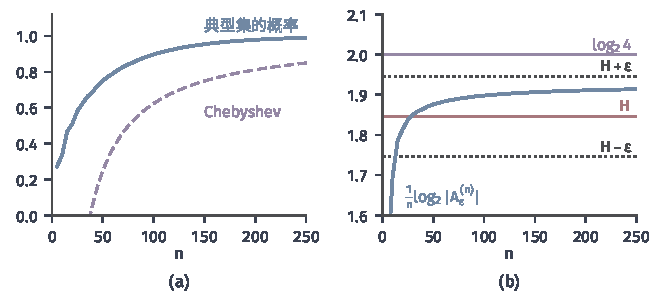
\includegraphics[width=110mm]{figures/07-probability/05-source-coding/matplotlib/lossless-typical-set/figure.pdf}
 \caption{贯穿例的典型集，$\varepsilon=0.1$，由类型枚举精确计算。(a)典型集的概率（蓝）与Chebyshev下界$1-\sigma^2/(n\varepsilon^2)$（紫色虚线），$\sigma^2=0.377$。(b)$\frac1n\log_2\lvert A_{\varepsilon}^{(n)}\rvert$（蓝），红线为$H$，灰色虚线为$H\pm\varepsilon$，紫线为全部块的$\log_24=2$。}
 \label{fig:lossless-typical-set}
\end{BookInlineFigure}

\paragraph{码率高于熵时可以做到}
典型集直接给出一种定长块编码：给典型集中的块逐个编号，另外留一个编号给所有非典型块。图~\ref{fig:lossless-typical-scheme}画出这一方案。

\begin{BookInlineFigure}
 \centering
 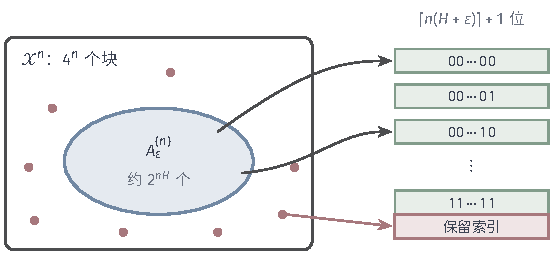
\includegraphics[width=94mm]{figures/07-probability/05-source-coding/tikz/lossless-typical-scheme/figure.pdf}
 \caption{用典型集构造定长块编码。左框为全部$4^n$个块，蓝色区域为典型集$A_{\varepsilon}^{(n)}$，约有$2^{nH}$个块；右侧绿格为等长的编号，每个典型块得到一个编号。红点为非典型块，全部送到红色的保留编号，解码时无法还原。}
 \label{fig:lossless-typical-scheme}
\end{BookInlineFigure}

\begin{theorem}[定长块编码的可达性]
\label{thm:lossless-fixed-achievability}
在定理~\ref{thm:lossless-aep}的条件下，对任意$R>H(X)$，存在一列定长块编码，其码率$R_n\leq R$（$n$充分大），错误概率$P_{\mathrm{e}}^{(n)}\to0$。
\end{theorem}

\begin{proof}
取$\varepsilon=(R-H(X))/2>0$。令编码映射把典型集中的块一一对应到编号$1,\dots,\lvert A_{\varepsilon}^{(n)}\rvert$，把其余块都映到编号$M_n=\lvert A_{\varepsilon}^{(n)}\rvert+1$；解码映射把前面的编号映回对应的典型块，把保留编号映到任意固定的块。由式~\eqref{eq:lossless-typical-upper}，
\[
 M_n<2^{n(H+\varepsilon)}+1\leq2^{n(H+2\varepsilon)}=2^{nR}
\]
在$n$充分大时成立，所以$R_n\leq R$。典型块都被正确还原，错误只可能发生在非典型块上，按式~\eqref{eq:lossless-error-prob}与式~\eqref{eq:lossless-typical-prob}，
\[
 P_{\mathrm{e}}^{(n)}\leq\mathbb{P}\bigl(X_{1:n}\notin A_{\varepsilon}^{(n)}\bigr)\leq\frac{\sigma^2}{n\varepsilon^2}\to0 . \qedhere
\]
\end{proof}

\paragraph{码率低于熵时做不到}
反过来，若码率低于熵，无论怎样选择要编号的块，错误概率都不能趋于零，实际上趋于$1$。

\begin{theorem}[定长块编码的逆定理]
\label{thm:lossless-fixed-converse}
在定理~\ref{thm:lossless-aep}的条件下，设$R<H(X)$，定长块编码满足$M_n\leq2^{nR}$。则$P_{\mathrm{e}}^{(n)}\to1$。
\end{theorem}

\begin{proof}
解码映射只有$M_n$个输出，能被正确还原的块组成集合
\[
 B_n=\{x_{1:n}:\ g_n(f_n(x_{1:n}))=x_{1:n}\},
\]
它的元素都在$g_n$的值域中，所以$\lvert B_n\rvert\leq M_n\leq2^{nR}$。取$\varepsilon=(H(X)-R)/2>0$，把正确还原的概率按是否典型拆开：
\[
 \mathbb{P}(X_{1:n}\in B_n)\leq\mathbb{P}\bigl(X_{1:n}\in B_n\cap A_{\varepsilon}^{(n)}\bigr)+\mathbb{P}\bigl(X_{1:n}\notin A_{\varepsilon}^{(n)}\bigr).
\]
第一项中每个块的概率小于$2^{-n(H-\varepsilon)}$，块的个数不超过$2^{nR}$，所以
\[
 \mathbb{P}\bigl(X_{1:n}\in B_n\cap A_{\varepsilon}^{(n)}\bigr)<2^{nR}\,2^{-n(H-\varepsilon)}=2^{-n\varepsilon}.
\]
第二项不超过$\sigma^2/(n\varepsilon^2)$。两项都趋于零，所以正确还原的概率趋于零，从而
\[
 P_{\mathrm{e}}^{(n)}=1-\mathbb{P}(X_{1:n}\in B_n)\to1. \qedhere
\]
\end{proof}

两个定理合起来说明，定长块编码能以趋于零的错误概率工作，当且仅当码率超过熵（$R=H$这一临界情形，上面的论证不作结论）。图~\ref{fig:lossless-fixed-rate-error}给出贯穿例中最好的定长码的错误概率：对给定的$M_n=\lfloor2^{nR}\rfloor$，编号给概率最大的$M_n$个块时错误概率最小。$R=1.95$时错误概率从$n=4$的$0.0157$降到$n=228$的$5.4\times10^{-5}$；$R=1.75$时，即使挑选最可能的块，错误概率仍从$0.160$升到$0.956$。

\begin{BookInlineFigure}
 \centering
 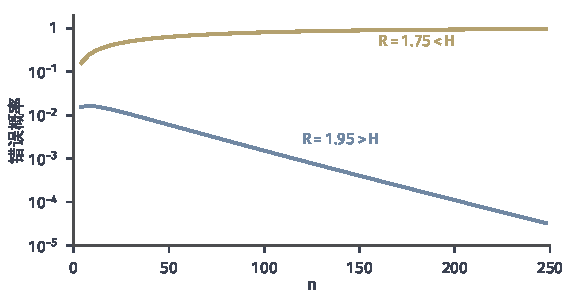
\includegraphics[width=96mm]{figures/07-probability/05-source-coding/matplotlib/lossless-fixed-rate-error/figure.pdf}
 \caption{贯穿例中码率为$R$的最优定长块编码的错误概率，纵轴为对数坐标。编码给概率最大的$\lfloor2^{nR}\rfloor$个块编号，其余块出错；数值由类型枚举精确计算。蓝线$R=1.95>H$，黄线$R=1.75<H$，$H=1.846$。}
 \label{fig:lossless-fixed-rate-error}
\end{BookInlineFigure}

\paragraph{错误来自哪里}
可达性定理中的错误全部来自非典型块，这些块合起来的概率很小。对单个块而言，结论是“要么精确还原，要么完全失败”：典型块精确还原，非典型块（例如$aa\cdots a$，以及$dd\cdots d$）一律出错。所以定理不能理解为“每条消息都能以接近熵的码率无损还原”。也不能理解为有限的$n$下错误概率已经可以忽略：贯穿例中$R=1.95$、$n=100$时错误概率仍有$1.5\times10^{-3}$。需要每条消息都还原时，应当用上一小节的变长块编码，它把这些罕见的块放到很长的码字里，而不是放弃它们。


\section{有限资源下的比较}
\label{sec:lossless-finite-resources}

前面的极限都在$n\to\infty$时成立，并且假定编码器知道真实的分布。实际选择编码方案时，块长有限，模型可能不准，码表要存储，编码要计算。本节在贯穿例上把各种方案放在同一组条件下比较：源分布相同，按每个源符号计算码长，解码要求分别写明。

\paragraph{几种方案的账本}
表~\ref{tab:lossless-comparison}列出贯穿例上的几种方案。平均码长一栏都按每源符号计；“最长码字”按一个编码单位（一个符号、一个块或整条消息）计；码本一栏是编码器与解码器需要共享的表的规模。

\begin{BookInlineTable}
 \centering
 \caption{贯穿例$p=(0.4,0.3,0.2,0.1)$上的几种编码方案，$H=1.846$。算术编码一行为图~\ref{fig:lossless-arith-length}中长$400$、长度已知的那条消息的实测值，码长小于消息自信息加$2$；定长块一行为图~\ref{fig:lossless-fixed-rate-error}中$R=1.95$、$n=100$的最优定长码。}
 \label{tab:lossless-comparison}
 \begin{tabular}{lcccc}
  \toprule
  方案 & 位/符号 & 最长码字 & 共享的表 & 错误概率\\
  \midrule
  定长$2$位 & $2$ & $2$ & 无 & $0$\\
  Huffman，$n=1$ & $1.900$ & $3$ & $4$项 & $0$\\
  Huffman，$n=2$ & $1.865$ & $6$ & $16$项 & $0$\\
  Huffman，$n=4$ & $1.853$ & $12$ & $256$项 & $0$\\
  Huffman，$n=6$ & $1.851$ & $19$ & $4096$项 & $0$\\
  算术编码 & $1.855$ & 随消息 & $4$个概率 & $0$\\
  定长块 & $1.95$ & $195$ & 排序规则 & $0.0015$\\
  \bottomrule
 \end{tabular}
\end{BookInlineTable}

从表中可以读出三点。第一，从$n=1$到$n=6$，块上Huffman码每符号只省下$0.049$位，码表却从$4$项增长到$4096$项，最长码字从$3$位增长到$19$位：越接近熵，每一点改进越贵。第二，算术编码只需共享四个概率，就达到了与$n=6$的块Huffman码相当的每符号码长；代价是每个符号要做乘法和区间比较，并且要处理有限精度。第三，定长块编码的码字最整齐，但要接受正的错误概率，不能用于必须逐条还原的场合。

\paragraph{码本的描述代价}
若编码器与解码器事先没有共享码表，码表本身也要传送。Huffman码由码长完全决定：把码长按从短到长排好，用第~\ref{sec:lossless-kraft}小节Kraft不等式充分性证明中的方法分配码字，得到的前缀码称为规范码，解码器只需知道每个块的码长。块长为$n$时要传送$4^n$个码长，每个码长用几位表示，总共是$4^n$乘以一个常数的位数。若消息只有$N$个符号，这一开销摊到每个符号上是$4^n/N$量级，块长增大带来的不到$1/n$位的收益，很快被它抵消。算术编码只需传送模型的四个概率（或模型的更新规则），描述代价与块长无关。

\paragraph{计算代价}
块上Huffman码的构造需要对$4^n$个块排序合并，计算量$O(4^n\cdot n)$；编码时查表，解码时在码树上逐位行走。算术编码不需要构造码表，每读一个符号做常数次乘法与比较，解码时要在累积概率表中找到$v$所在的子区间，字母表较大时用二分查找。两者都是每个源符号常数量级的工作，但Huffman码的常数随块长指数增长，算术编码的常数与消息长度无关。

\paragraph{模型失配的代价}
设计编码时用的分布$q$称为模型，信源的真实分布是$p$，两者可能不同。码长是按$q$设计的，平均码长却要按实际出现的频率，即按$p$加权。定理~\ref{thm:lossless-entropy-bound}证明中的分解在这里给出精确的账目。

\begin{theorem}[失配的Shannon码]
\label{thm:lossless-mismatch}
设$p,q$是$\mathcal{X}$上的概率质量函数，各$p(x)>0$、$q(x)>0$，且$q(x)<1$对每个$x$成立。按模型$q$取码长$\ell(x)=\lceil-\log_2q(x)\rceil$的前缀码，在真实分布$p$下的平均码长满足
\begin{equation}
 H(p)+D_{\mathrm{KL}}(p\Vert q)\leq\sum_xp(x)\ell(x)<H(p)+D_{\mathrm{KL}}(p\Vert q)+1 ,
 \label{eq:lossless-mismatch}
\end{equation}
其中$H(p)$是$p$的熵。
\end{theorem}

\begin{proof}
码长满足Kraft不等式，理由同定理~\ref{thm:lossless-entropy-bound}，所以这样的前缀码存在。对每个$x$，
\[
 -\log_2q(x)=-\log_2p(x)+\log_2\frac{p(x)}{q(x)} .
\]
按$p$加权求和，右边的平均是$H(p)+D_{\mathrm{KL}}(p\Vert q)$。而$-\log_2q(x)\leq\ell(x)<-\log_2q(x)+1$，乘$p(x)$求和即得式~\eqref{eq:lossless-mismatch}。
\end{proof}

所以模型失配的代价是KL散度$D_{\mathrm{KL}}(p\Vert q)$：按错误的概率分配码长，每符号平均多付这么多位。左侧的不等式说明这部分损失无法靠取整挽回；它与整数码长的冗余是两笔不同的账。

图~\ref{fig:lossless-mismatch}在贯穿例上让模型从$p$逐渐变到反序的$r=(0.1,0.2,0.3,0.4)$，即$q_t=(1-t)p+tr$。$t=0$时模型准确，Huffman码平均$1.9$位；$t=1$时按$r$设计的Huffman码给$a$三位、$d$一位，按真实概率加权，
\[
 0.4\times3+0.3\times3+0.2\times2+0.1\times1=2.6 ,
\]
比准确模型多$0.7$位，比定长码还差。此时$D_{\mathrm{KL}}(p\Vert r)=0.658$，Shannon码平均$3.1$位，落在式~\eqref{eq:lossless-mismatch}给出的$[2.505,3.505)$中。另一个特例是均匀模型：码长都是$2$，平均码长$2$恰好等于
\[
 H(p)+D_{\mathrm{KL}}(p\Vert u)=1.846+0.154 .
\]

\begin{BookInlineFigure}
 \centering
 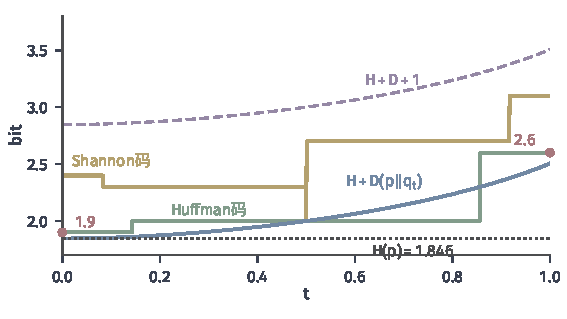
\includegraphics[width=96mm]{figures/07-probability/05-source-coding/matplotlib/lossless-mismatch/figure.pdf}
 \caption{模型失配。真实分布$p=(0.4,0.3,0.2,0.1)$，设计模型$q_t=(1-t)p+t\,r$，$r=(0.1,0.2,0.3,0.4)$。纵轴为按$p$计算的平均码长：黄线为按$q_t$设计的Shannon码，绿线为按$q_t$设计的Huffman码；蓝线为$H(p)+D_{\mathrm{KL}}(p\Vert q_t)$，紫色虚线为再加$1$，灰色点线为$H(p)$。红点为两端的Huffman码平均码长。}
 \label{fig:lossless-mismatch}
\end{BookInlineFigure}

图中Huffman码的曲线是阶梯形：模型稍有偏差时，码长的整数取值往往不变，平均码长也不变；偏差累积到改变码树时才跳一级。在$t$约从$0.5$到$0.86$之间，按$q_t$设计的Huffman码甚至落在蓝线下方，这并不矛盾：式~\eqref{eq:lossless-mismatch}只约束Shannon码，任何码的平均码长只受$H(p)$约束。

\paragraph{失配与不一致是两回事}
模型失配时，编码器与解码器用同一个$q$，码仍然唯一可译，每条消息都正确还原，只是平均更长。另一种错误是两端不一致：编码器与解码器用了不同的码表或不同的概率。这时码长没有变，解码结果却错了。

两个例子都来自本章的码表。第~\ref{sec:lossless-model}节的码表中$c\mapsto110$、$d\mapsto111$，第~\ref{sec:lossless-huffman}小节Huffman过程得到的码表中$c\mapsto111$、$d\mapsto110$，两者平均码长相同。若编码器用前者把$abac$编成$0100110$，解码器却用后者，读出的是$abad$。算术编码也一样：编码器按$p=(0.4,0.3,0.2,0.1)$把$abac$编成$00110010$，若解码器误用$(0.3,0.4,0.2,0.1)$，则从$v=0.1953$逐步读出
\[
 a,\quad b,\quad c,\quad c ,
\]
得到$abcc$。

所以评价一个方案要分开两件事：在两端一致的前提下，模型偏离真实分布会使平均码长增加$D_{\mathrm{KL}}(p\Vert q)$左右；两端不一致则破坏可解码性，与平均码长无关。前者靠更好的模型改进，后者要靠严格共享的规则（码长表、符号顺序、概率与取整方式）来避免。


\section{本章小结}
\label{sec:lossless-summary}

本章从“常见符号用短码能省多少”出发，回答了三个层次的问题，每个层次对应各自的约束。

第一层是可解码性。码字互不相同还不够，拼接以后必须能唯一地切开。前缀码让解码器在码树上即时断开码字；唯一可译码允许码字互为前缀，但要付出解码延迟。Kraft–McMillan不等式说明两者能实现的码长集合相同，都由$\sum_x2^{-\ell(x)}\leq1$刻画；这一条件约束的是码长，码字仍须按保证前缀性的方法分配。

第二层是平均码长的最优性。对至少两个符号有正概率的信源，唯一可译码的平均码长不小于熵，等号要求每个码长恰为自信息；按自信息取整的Shannon码平均码长小于熵加一。平均码长与熵之差拆成两部分：码长暗含的概率与真实概率的KL散度，以及Kraft不等式未取等号所浪费的空间。冗余是加权平均，个别符号的码长可以短于自信息。确定源只有在消息长度已知时才能零码长。

第三层是可执行的构造与渐近极限。Huffman编码逐次合并概率最小的两个符号，对给定有限符号表求出平均码长最短的前缀码，贯穿例中为$1.9$位，熵为$1.846$位。

算术编码把整条消息对应到长度等于其概率的区间，码长不超过自信息加两位，需要约定终止规则，两端须使用完全相同的模型与取整方式，模型给实际符号零概率时无法编码。

把符号组成块之后有两种资源制度：零错误的变长块编码使每符号冗余小于$1/n$，代价是最坏码长和码本随块长增长；允许错误的定长块编码借助渐近均分性和典型集，码率高于熵时错误概率趋于零，低于熵时趋于一，失败来自被放弃的小概率块。

在有限资源下，块长带来的收益很快被码本与计算代价抵消；模型失配使平均码长增加KL散度，两端不一致则直接造成解码错误。第~\ref{chap:quantization}章不再要求精确还原，允许重构值与原值有偏差，研究把连续取值装进有限个格子的量化器，并用失真来衡量这种偏差；量化后的格子编号仍可用本章的方法无损压缩。

